\section{Results}

To test the accuracy of our model, we perform Leave One Out (LOO) Cross Validation. This form of cross validation involves using one observation as the validation set and the remaining observations as the training set. This is repeated for all combinations of training sets, allowing every observation to act as a validation set. For our analysis an observation is one set of configurations. For example, consider five sets of configurations: A through E. We pick A as the validation set and train the model on all other configurations.\\

For a single test, our program will now "walk through" rebuilding configuration A token-by-token, starting from the first keyword. At every step, we invoke our model and compare our predictions against the actual tokens in A. If the model generates the correct prediction within the top three results, we mark a token completion to be successful. We tally up the number of model invocations and the number of correct predictions.\\
 
\begin{figure}[H]
	\centering
	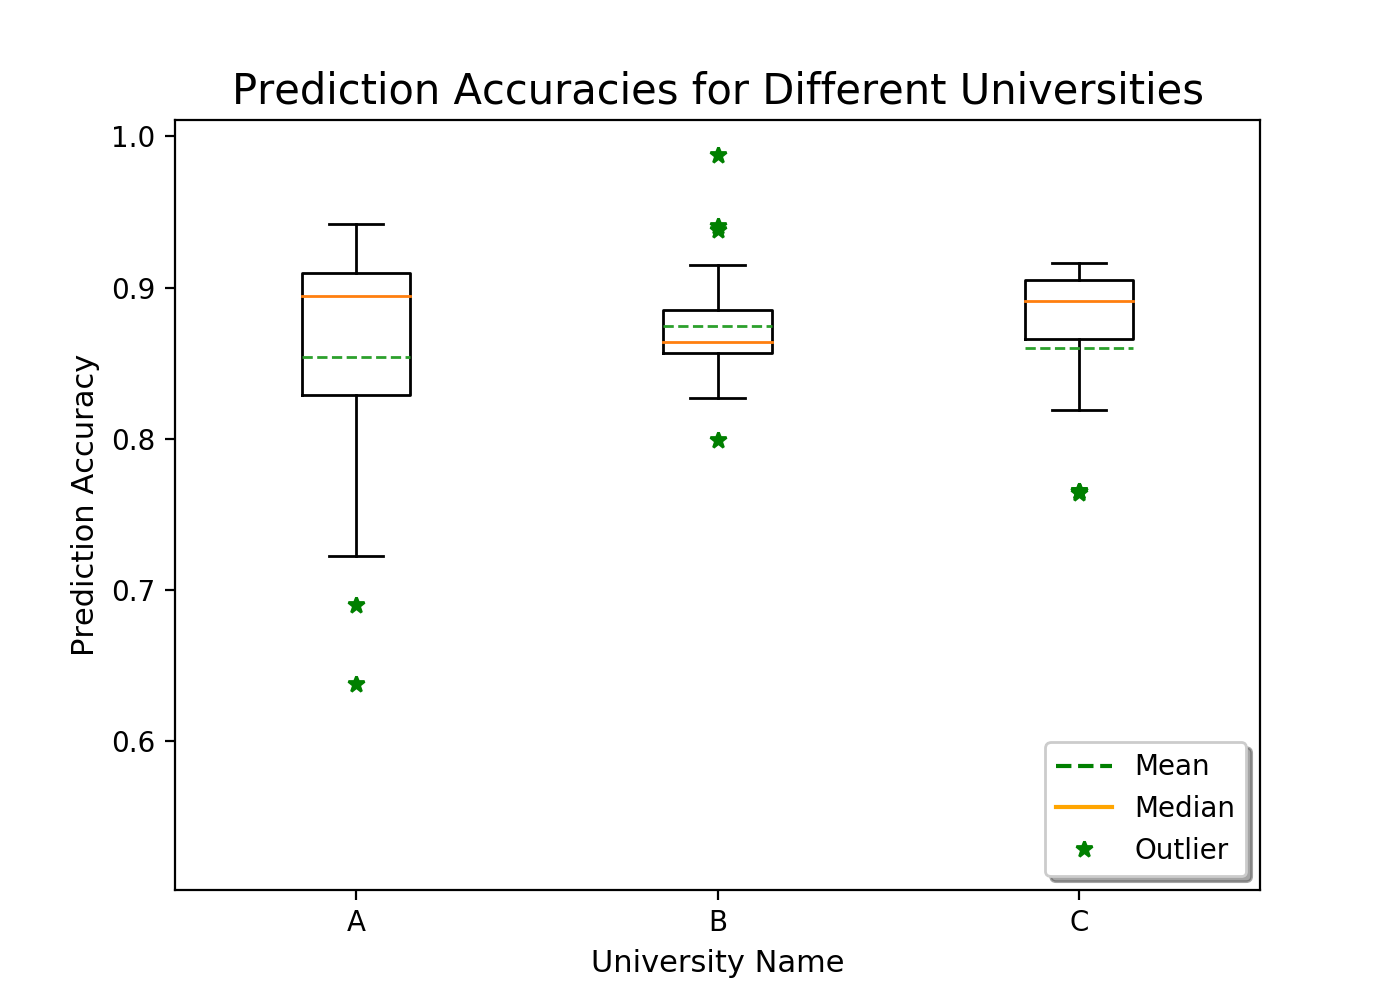
\includegraphics[width=5in]{uni_analysis.png}
	\caption{Overall accuracy of the model for each set of university configurations used as the validation set.}
\end{figure}

In the figure shown above, the the x-axis shows the name of the three anonamyzed universities used, and prediction accuracies on the y-axis. The box plot is supposed to highlight the average (green dotted line), median (orange line) and upper ($Q_U$) and lower quartiles ($Q_L$). The box itself marks the Inter Quartile Range (IQR). The outliers (green stars) are all the data points that lie outside $Q_L - 1.5*IQR$ and $Q_U+1.5*IQR$.\\

Initially, without any preprocessing and subnet removal, we observed a maximum accuracy of 85\% and an average of 65\%. Our results in the figure above are after preprocessing the data and we now see accuracies as high as 93\%, and an average of 81\%. These results are very promising as we see a significant jump in accuracy from simple refinements to the model. More placeholders would improve accuracies even further but with diminishing returns.

\begin{figure}[H]
	\centering
	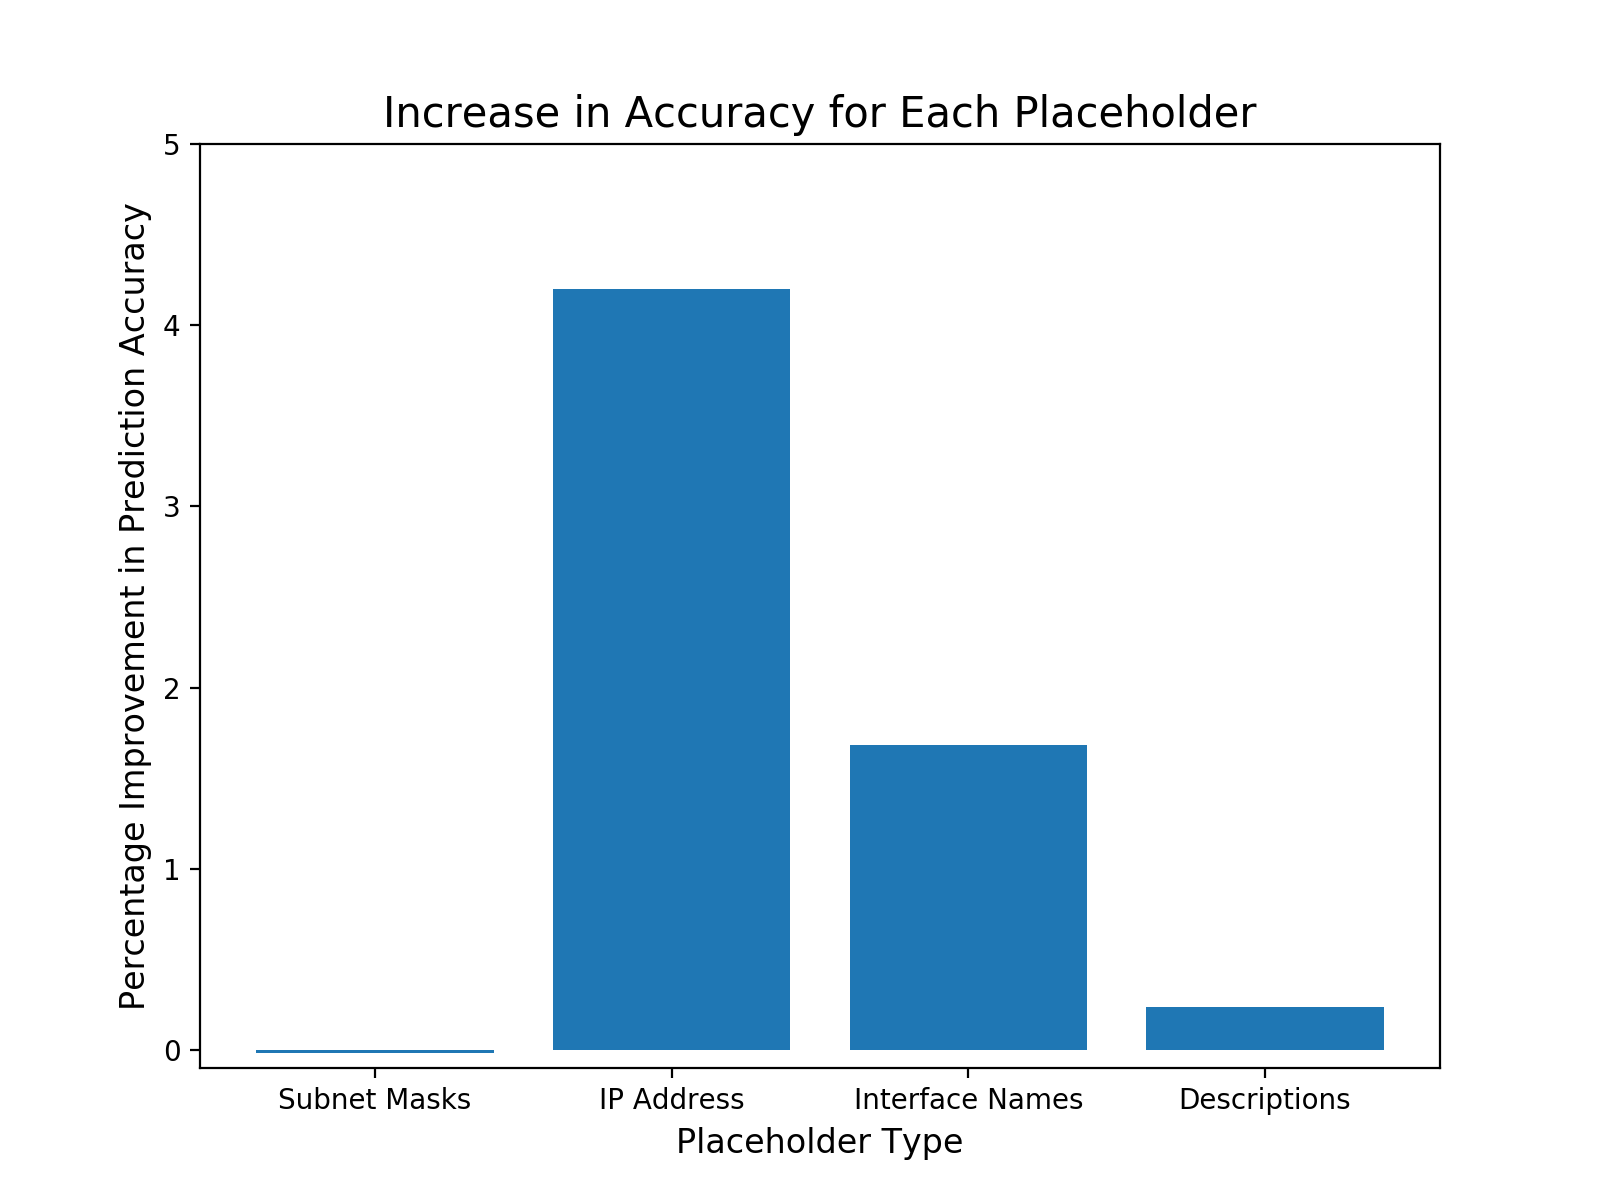
\includegraphics[width=\textwidth]{placeholders.png}
	\caption{Overall accuracy of the model for each set of university configurations used as the validation set.}
\end{figure}


\subsection{Evaluations}

There were a myriad of analyses we performed in order to test the efficacy of an ngram-based engine as described in the previous section. In this paper we discuss some which produced interesting results.

\subsection{Role-Based}

\begin{figure}[H]
	\centering
	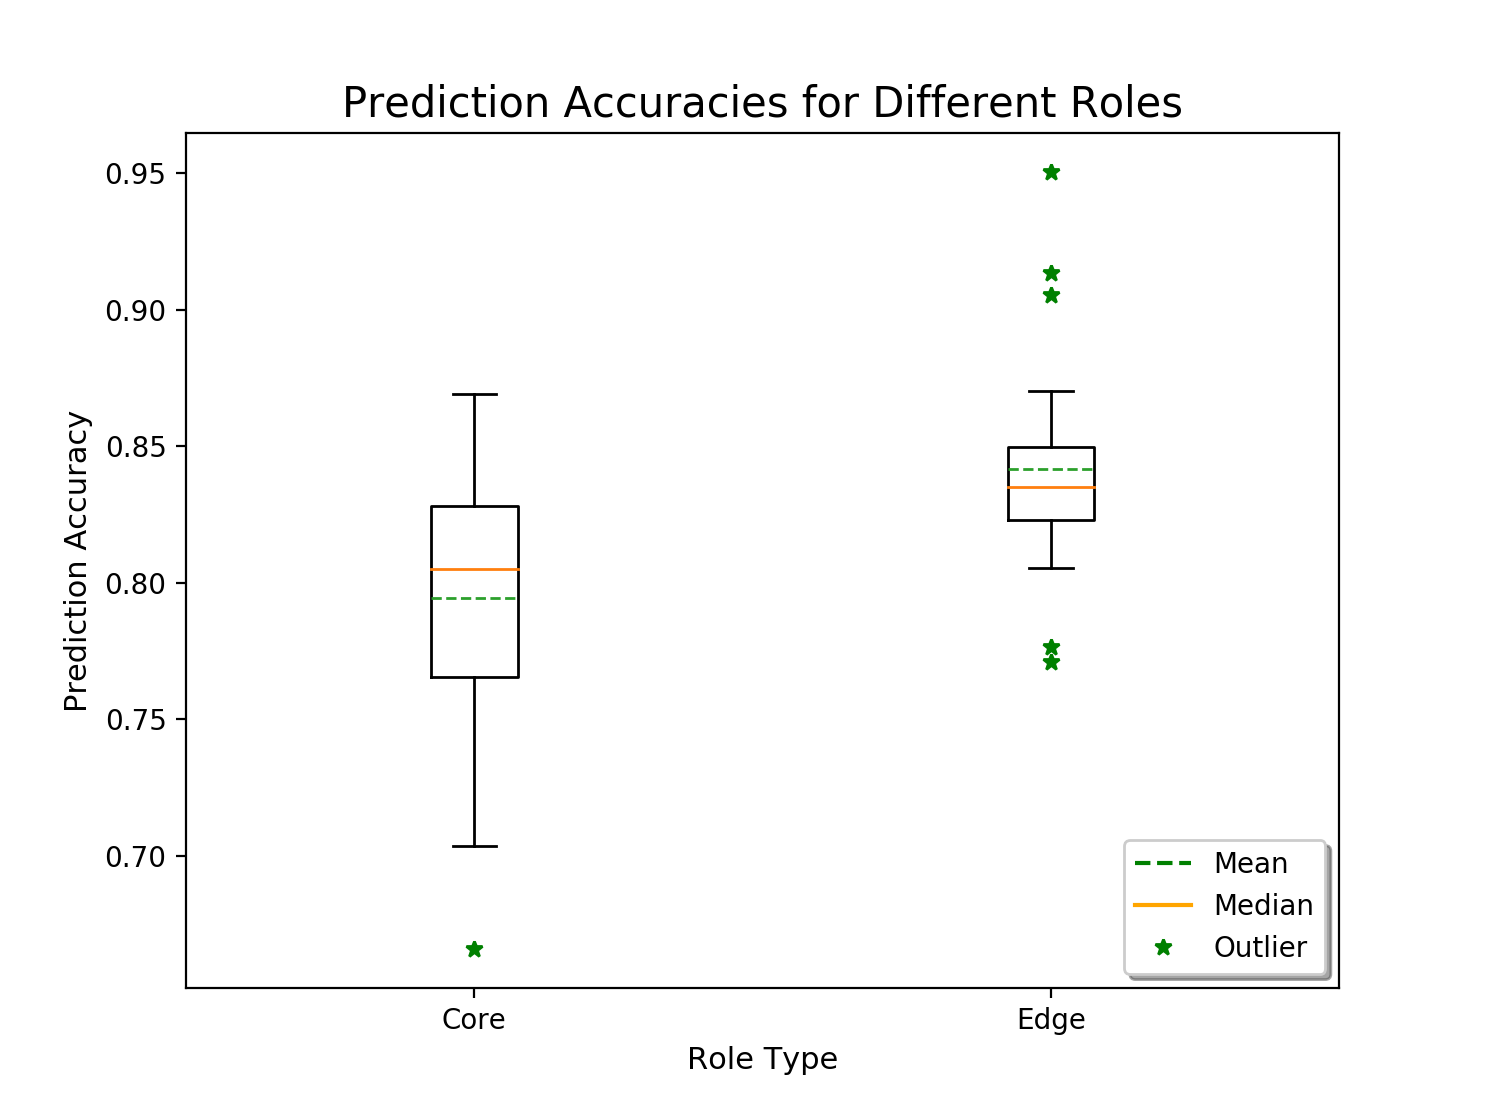
\includegraphics[width=\textwidth]{roles.png}
	\caption{Accuracies of models were trained on core and edge routers only.}
\end{figure}

Training models based on different roles improved accuracies in some cases but not others.

\subsection{histories}

As we had extensive data from University A's version control system, we analyzed the effect of selecting configurations across time on prediction accuracies. The x-axis of the graph shows the number of months we chose to train on.

\subsection{Per-Stanza}

\subsection{No starting datat}